\documentclass[]{standalone}%
%
\usepackage{tikz}%
%
\definecolor{TUMBlack}{cmyk}{0,0,0,1}%
\definecolor{TUMBlue}{cmyk}{1,0.43,0,0}%           Pantone 300
\definecolor{TUMBlue1}{cmyk}{1,0.57,0.12,0.7}%     Pantone 540
\definecolor{TUMBlue2}{cmyk}{1,0.54,0.04,0.19}%    Pantone 301
\definecolor{TUMBlue3}{cmyk}{0.65,0.19,0.01,0.04}% Pantone 542
\definecolor{TUMBlue4}{cmyk}{0.42,0.09,0,0}%       Pantone 283
\definecolor{TUMOrange}{cmyk}{0,0.65,0.95,0}%
\definecolor{TUMGreen}{cmyk}{0.35,0,1,0.2}%
%
\begin{document}%
%
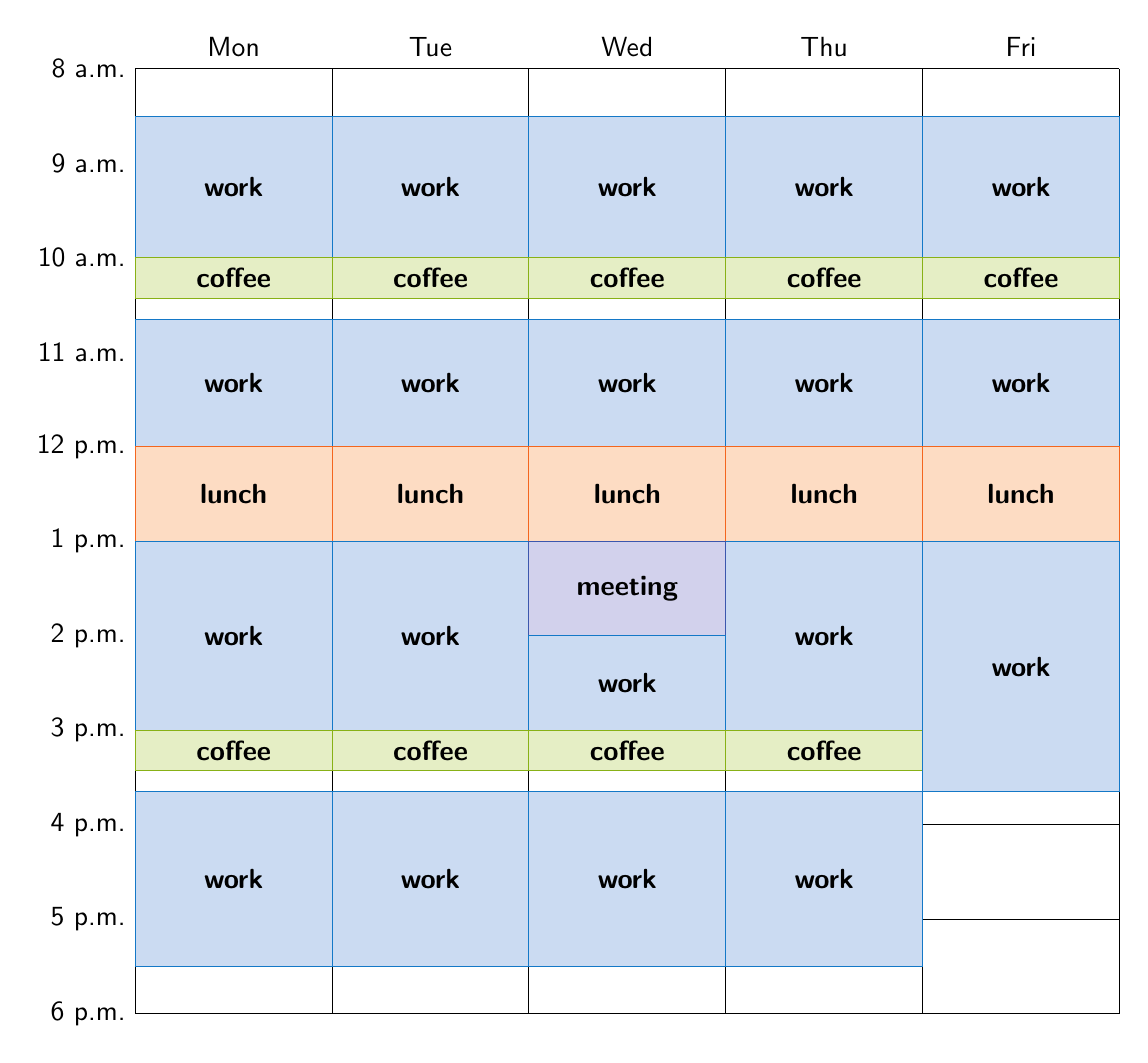
\begin{tikzpicture}[font=\sffamily,
    declare function={Mon=0;Tue=1;Wed=2;Thu=3;Fri=4;
    hscale=2.5;vscale=1.2;tmin=8;tmax=18;},
    yscale=-1,x=hscale*1cm,y=vscale*1cm,
    course color/.code={\colorlet{coursecolor}{#1}},
    course color=TUMBlue,
    course/.style args={#1 from #2 to #3}{%
            draw=coursecolor,fill=coursecolor!20,
            at={(#1,#2)},align=center,
            node font=\bfseries,
            anchor=north west,outer sep=0pt,
            minimum width=hscale*1cm,
            minimum height={abs(#3-#2)*vscale*1cm}}]
    \pgfmathtruncatemacro{\tmin}{tmin}%
    \pgfmathtruncatemacro{\tnext}{tmin+1}%
    \pgfmathtruncatemacro{\tmax}{tmax} 
    \draw[xstep=hscale*1cm,ystep=vscale*1cm]  (0,tmin) grid (5,tmax);
    \path foreach \X  [count=\Y] in
       {Mon,Tue,Wed,Thu,Fri}
       {(\Y-0.5,8) node[above,text depth=0.25ex]{\X} }
       foreach \X [parse=true] in {\tmin,\tnext,...,\tmax}
       {(0,\X) node[left]{\ifnum\X<12\relax
       \X\ a.m.%
       \else
       \ifnum\X=12\relax
          12\ p.m.%
       \else
          \the\numexpr\X-12\relax\ p.m.%
       \fi
       \fi} }; 
    \path 
    foreach \X in {Mon,Tue,Thu}{
          node[course={\X} from 8.5 to 10]{work}
          node[course color=TUMGreen,course={\X} from 10 to 10.25]{coffee}
          node[course={\X} from 10.65 to 12]{work}
          node[course color=TUMOrange,course={\X} from 12 to 13]{lunch}
          node[course={\X} from 13 to 15]{work}
          node[course color=TUMGreen,course={\X} from 15 to 15.25]{coffee}
          node[course={\X} from 15.65 to 17.5]{work}
       }
   
    foreach \X in {Wed}{
          node[course={\X} from 8.5 to 10]{work}
          node[course color=TUMGreen,course={\X} from 10 to 10.25]{coffee}
          node[course={\X} from 10.65 to 12]{work}
          node[course color=TUMOrange,course={\X} from 12 to 13]{lunch}
          node[course color=TUMBlue3!40!blue,course={\X} from 13 to 14]{meeting}
          node[course={\X} from 14 to 15]{work}
          node[course color=TUMGreen,course={\X} from 15 to 15.25]{coffee}
          node[course={\X} from 15.65 to 17.5]{work}
       } 
       
       foreach \X in {Fri}{
          node[course={\X} from 8.50 to 10]{work}
          node[course color=TUMGreen,course={\X} from 10 to 10.25]{coffee}
          node[course={\X} from 10.65 to 12]{work}
          node[course color=TUMOrange,course={\X} from 12 to 13]{lunch}
          node[course={\X} from 13 to 15.65]{work}
       } ;
 \end{tikzpicture}
%
\end{document}%
%